
\documentclass{amsart}

\usepackage[latin1]{inputenc}
\usepackage{caption, subcaption}
\usepackage{amsfonts, amsmath, thmtools}
\usepackage{fullpage}
\usepackage[pagebackref=false,bookmarksopen=false,colorlinks,citecolor=black,linkcolor=violet]{hyperref} 
\usepackage{multirow,xcolor,pifont,varwidth}
\usepackage{tikz}
\usetikzlibrary{matrix,shapes,arrows,positioning,chains,calc}

\newcommand{\comment}[1]{\marginpar{\color{red}{\Huge$*$}}\mbox{}{\sf\color{red}[#1]}}

\makeatletter
\renewcommand*{\@makefnmark}
    {\hbox{\@textsuperscript{\scalebox{1}{\normalfont\@thefnmark}}}}
\makeatother

%--------------------------------------
% Theorem definitions
%--------------------------------------
\newtheorem{theorem}{Theorem}[section]
\newtheorem{lemma}[theorem]{Lemma}
\newtheorem{conjecture}[theorem]{Conjecture}
\newtheorem{cor}[theorem]{Corollary}
\newtheorem{prop}[theorem]{Proposition}
\newtheorem{quest}{Question}
\newtheorem*{xtheorem}{Theorem}
\theoremstyle{remark}
\declaretheorem[name=Example,qed={\lower-0.3ex\hbox{$\triangleleft$}}]{example}
\newtheorem{remark}{Remark}


\author{Stephen Melczer, Taras Mychaskiw and Yi Zhang}

\title{Password Authenticated Key Exchange:\\ From Two Party Methods to Group Schemes}

%\keywords{Lattice path enumeration, D-finite, diagonal, analytic
%  combinatorics in several variables, Weyl chambers}   % seems legit


\begin{document}

\begin{abstract}
This project investigates password authenticated key exchange methods (PAKEs), and variants involving many agents:
group password authenticated key exchange methods (GPAKEs).  In 
particular, after surveying classical information on two party PAKEs we detail the so-called `fairy ring dance' method recently described by 
Hao et. al.~\cite{HaYiChSh15} which allows for the extension of two party password authenticated key exchange 
methods (PAKEs) with key confirmation to a group setting with an arbitrary number of users without
increasing round complexity (the computational complexity, of course, increases with the number of users).  
This paper presents two new GPAKEs constructed through these means, based on the 
Dragonfly and PAK/PPK two party protocols, and includes timings comparing them to previous GPAKEs of
Hao et. al.~\cite{HaYiChSh15}.
\end{abstract}

%------------------------------------------------------
\maketitle
%------------------------------------------------------

%%%%%%%%%%%%%%%%%%%%%
% Introduction
%%%%%%%%%%%%%%%%%%%%%

\section{Introduction}

Since their introduction in the 1990s, password-authenticated key exchange (PAKE) methods -- 
also known as password-authenticated key agreement methods -- have become popular for their 
ability to allow agents sharing a (typically low entropy) password to securely establish shared 
cryptographic keys (see Bellovin and Merritt~\cite{BeMe92} or Jablon~\cite{Ja96} for early examples, 
and Hao and Ryan~\cite{HaRy2010} for a more recent paper).  Although they have been around for decades, 
most research on PAKEs has focused on key establishment between two parties.  For our project, we 
have studied the problem of establishing Group PAKEs (GPAKEs) -- that is, using a low entropy password 
shared between many agents to set up cryptographic keys.  This has modern applications with the rise
of the so-called `Internet of Things', where many consumer devices connected through a local Internet 
connection wish to securely communicate (such schemes would allow, for instance, secure communication 
between a smart television, DVD player, and cable box after their owner inputs a short shared password 
into each upon purchase).
\\

The major issue in designing an efficient GPAKE is to minimize the number of rounds of communication 
between the agents involved, as the latency of such a protocol is determined by the slowest responder 
in each round.  A recent pre-print of Hao et. al.~\cite{HaYiChSh15} proposes a construction which 
allows for the extension of any secure two-party PAKE  with key confirmation to a multi-party PAKE,
without adding any extra rounds of communication (if the underlying two-party PAKE only allows for
key authentication, then the associated GPAKE has one extra round of communication).  The authors continue 
on to give two explicit schemes following from this template: SPEKE+ (using two rounds of communication, 
adapted from the SPEKE~\cite{Ja96} protocol) and J-PAKE+ (using three rounds of communication, adapted from 
the J-PAKE~\cite{HaRy2010} protocol).
\\ 

The structure of this document is as follows: Section~\ref{sec:PAKE} begins by giving a survey of classical 
two-party PAKEs -- including explicit descriptions of the PAKEs which will be extended into the group 
setting.  Section~\ref{sec:GPAKE} 
starts with a description of the theoretical methodology developed by Hao et. al.~\cite{HaYiChSh15} to extend 
two-party PAKEs into a group setting.  After this general background, we give two explicit GPAKEs 
(SPEKE+ and J-PAKE+) constructed by Hao et. al. using this methodology, followed by two explicit GPAKEs 
which we have derived through the same means (a group variant of the IEEE 802.11-2012 standard Dragonfly 
protocol~\cite{Ha15}, and a variant of the PAK/PPK protocol \cite{BoMaPa00}).  Security properties of these
GPAKEs follow from the security properties of the underlying two party PAKES, in a manner described by Hao et. al.~\cite{HaYiChSh15} 
and in Section~\ref{sec:GPAKE} of this document.  In Section~\ref{sec:Implementation} we test the practical efficacy of our new methods 
against the Java implementations of SPEKE+ and J-PAKE+ given by Hao et. al.~\cite{HaYiChSh15}.  Section~\ref{sec:Conclusion} 
concludes with an overview of these results and possible directions for future work.
\\ 

The main original contributions found in this project come from the two new group PAKEs we have constructed 
-- see sub-Sections~\ref{sec:Dragon} and~\ref{sec:PPK} -- and timings 
which compare these methods against previous Java implementations of SPEKE+ and J-PAKE+ (the code for this project is 
available at \url{https://github.com/twentylemon/gpake}).  
We also survey the relevant background material on Zero Knowledge Proofs and classical PAKEs missing from
Hao et. al.~\cite{HaYiChSh15} (which had constrained space as a conference abstract), and fixed some minor 
Java implementation oversights which could cause the timings in that paper to be slightly inaccurate.

%%%%%%%%%%%%%%%%%%%%%
% Two Party Schemes
%%%%%%%%%%%%%%%%%%%%%

\section{Two Party Password-Authenticated Key Exchange (PAKE)
{\protect\footnote{The background information in this section, and details about SPEKE and J-PAKE, are mainly based on the presentation 
 in Hao and Ryan~\cite{HaRy2010}. The information on the Dragonfly protocol was taken from Harkins~\cite{Ha15} and Clarke and Hao~\cite{Ha2014}.  
 The sub-section about PAK/PPK is based on the work of Boyko et. al.~\cite{BoMaPa00}.}}}
\label{sec:PAKE}
 
 The genesis of password-authenticated key exchange is widely credited to the 1992 work of Bellovin and 
 Merrit~\cite{BeMe92}, whose protocol -- known as Encrypted Key Exchange, or EKE, for short -- came to 
 be known as the first PAKE (previous password based protocols, like the one proposed in 1989 by Lomas et.al.~\cite{LoGoSaNe89}, 
 contained key features of PAKEs such as the offline dictionary attack resistance detailed below, although they still relied on
 one party having another's public key).  All PAKEs aim for two main goals: to require their users to provide a zero 
 knowledge proof of a short password known to both parties \emph{a priori} (that is, before the protocol 
 has begun) and to leverage knowledge of this password to facilitate an authenticated key exchange.  As 
 password are assumed to be low entropy -- for instance, they are often treated as human memorable 
 passwords (typically assumed to be approximately 20-30 bits of entropy) -- if the passwords 
 themselves were broadcast they would need to be protected, for instance using SSL.  This would require Public 
 Key Infrastructure, such as a Trusted Authority / Certificate Authority to maintain public keys, which can be expensive.
 The ability to work around such infrastructure is often the point of PAKE protocols, which essentially use
 pre-established shared knowledge (of the common password) as an alternative to Trusted Authorities.
 \\

 Indeed, it is somewhat miraculous that PAKEs -- which transform a low entropy shared secret into a 
 much larger and more complicated shared key -- exist at all.  Although the EKE protocol of Bellovin and 
 Merrit was later shown to have weaknesses (see Jaspan~\cite{Ja96}, for example) its great contribution was 
 to show that such schemes can be achieved.  Due to its historical significance, we outline the Diffie-Hellman
 variant of the method here (an RSA variant, also by Bellovin and Merrit, was later shown to be insecure).  
 Given a symmetric encryption function $[\cdot]_\pi$ which uses a password $\pi$ shared
 by agents Alice and Bob as a key, the algorithm does the following:
 \\

\begin{figure}[h]
\textbf{Setup:} Let $\alpha$ be a primitive root of $\mathbb{Z}_p$
    \begin{tikzpicture}
        \matrix (m)[matrix of nodes, column sep=1cm, column 2/.style={minimum width=1.5cm}, nodes in empty cells]{
            Alice                                       &                   & Bob                                       \\
            randomly choose $x_a \in \mathbb{Z}_p^*$    &                   & randomly choose $x_b \in \mathbb{Z}_p^*$  \\
                                                        & $[\alpha^{x_a}]_\pi$&                                           \\
            									        & $[\alpha^{x_b}]_\pi$&       									\\
            Compute $K = \alpha^{x_a \cdot x_b}$ & & Compute $K = \alpha^{x_a \cdot x_b}$ \\
        };

        % draw the nodes - these are 1-based indicies on the matrix called `m`, ie to draw in (x,y), reference it as `m-x-y`
        \draw[shorten <=-1.5cm,shorten >=-1.5cm] (m-1-1.south east)--(m-1-1.south west);    % underline "Alice"
        \draw[shorten <=-1.5cm,shorten >=-1.5cm] (m-1-3.south east)--(m-1-3.south west);    % underline "Bob"
        \draw[shorten <=-1cm,shorten >=-1cm,-latex] (m-3-2.south west)--(m-3-2.south east); % arrow below sending alpha^x_a
        \draw[shorten <=-1cm,shorten >=-1cm,-latex] (m-4-2.south east)--(m-4-2.south west); % arrow below sending alpha^x_b
    \end{tikzpicture}
    \caption{The flow diagram for EKE}
    \label{fig:EKE}
\end{figure}

At the end, both Alice and Bob share the key $K = \alpha^{x_a \cdot x_b}$.  The weaknesses of the algorithm 
stems from the issues discussed above: as the password has low entropy in order for the scheme to be 
secure the input into $[\cdot]_{\pi}$ must essentially look like a random number.  But a 1024 bit number 
modulo $p$ is not random, and a passive attacker can try candidate passwords $\pi'$ to attempt to decipher 
$\left[\alpha^{x_a}\right]_{\pi}$ and immediately rule out any passwords giving a result in the range $[p,2^{1024}-1]$.
\\

Although EKE has this, and other, weaknesses, it was extremely influential and its general characteristics are 
reflected in many of the more advanced protocols we outline below (there is also a minor variant known as EKE2,
which was shown to be secure by Bellare, Pointcheval, and Rogaway~\cite{BePoRo00}).  Before giving these methods, we must outline 
what constitutes a good measure of security for a PAKE. To begin, a secure two party PAKE satisfies each of the following properties
coming from the security of general key exchange protocols:
\\

\begin{itemize}
 \item[] \textbf{(Offline dictionary attack resistance)}
 \item[] The PAKE does not leak any information to a passive or active attacker which can be 
 used by the attacker to determine the password through a brute force search (the protocol 
 cannot reveal a hash of the password, for instance).
 \item[]
 \item[] \textbf{(Forward secrecy for established keys)}
 \item[] If the password is disclosed, past session keys cannot be computed by an attacker.  
 This implies that a \emph{passive} attacker who knows the password cannot learn a session 
 key by observing communication between Alice and Bob (of course, an active attacker could 
 establish a shared key with one of the participants as he would have access to all of their 
 secret information).
 \item[]
 \item[] \textbf{(Known session security)}
 \item[] Even if an attacker learns all session specific secrets of a protocol in progress, these secrets do not reveal 
 any information about other established sessions.
  \item[]
 \item[] \textbf{(Online dictionary attack resistance)}
 \item[] An active attacker can only test one password per protocol execution (this is the 
 best that we can reasonably assume, as any attacker can randomly guess a password and 
 run the protocol -- at some point the key must be confirmed, either explicitly through the 
 PAKE or when the key is used in some other protocol, and the attacker will know whether or
 not his guess was correct).  This is sometimes relaxed (for instance, in the proof of SPEKE given
 by MacKenzie~\cite{Mac01}) to restricting the attacker to at most a small constant number of tests
 per protocol execution.
\item[]
\end{itemize}

 %These properties are illustrated in sub-Section~\ref{sec:JPAKE} when we outline their proof
 %for the J-PAKE protocol. 
 In the modern literature, a full proof of security essentially requires showing that an attacker
 can only gain information about established keys or a shared password if he is active, and that even an active
 attacker can gain extremely little information (for instance, can only guess one password per protocol execution).
 The formal model of Bellare, Pointcheval, and Rogaway~\cite{BePoRo00} is commonly used as a standard, and three of the 
 four PAKEs discussed later in this section have been proven secure -- under various assumptions, see Figure~\ref{fig:Compare} -- in
 this model (the fourth, which is the Dragonfly protocol of sub-Section~\ref{sec:Dragon}, we include despite a formal 
 proof of security as it is an IEEE 802.11-2012 standard).  We refer an interested reader to the work of 
 Abdalla et. al.~\cite{AbdBenMac15} and MacKenzie~\cite{Mac02} for in-depth discussions of PAKE security and attack models.

 %\begin{figure}[ht]
 %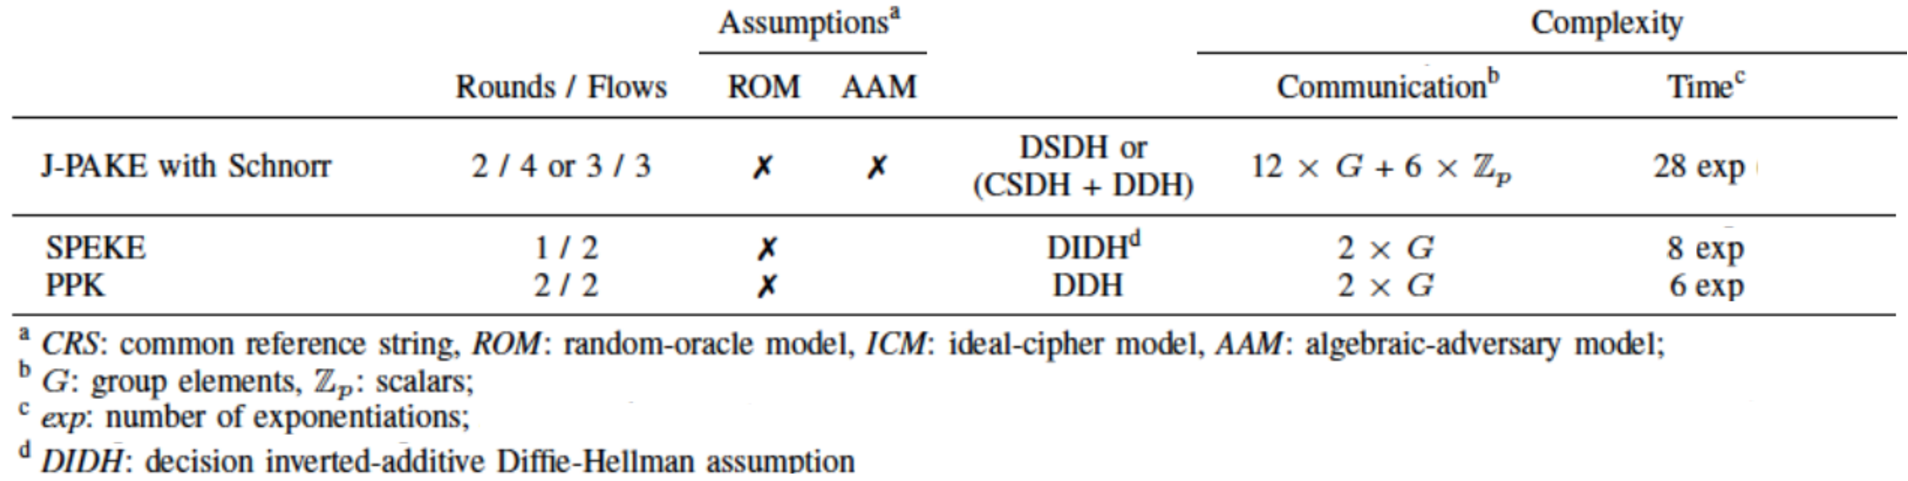
\includegraphics[width=\linewidth]{Comparisons.pdf}
 %\caption{Table taken from  Abdalla et. al.~\cite{AbdBenMac15} comparing the security assumptions and complexity of the 
 %methods discussed below}
 %\label{fig:Compare}
 %\end{figure}

\begin{table}[h]
\begin{tabular}{c|c|c|c|c}
                  & Rounds / Flows & Assumptions    & Communication\footnotemark                         & Time               \\ \hline\hline
J-PAKE w/ Schnorr & 2 / 4          & ROM, AAM, DSDH & $12 \times G + 6 \times \mathbb{Z}_p$ & 28 exponentiations \\
SPEKE             & 1 / 2          & ROM, DIDH      & $2 \times G$                            & 8 exponentiations  \\
PPK               & 2 / 2          & ROM, DDH       & $2 \times G$                            & 6 exponentiations       
\end{tabular}
\vspace{0.2in}

\caption{Table comparing the security assumptions needed for the 
 provably secure methods (in the BPR model) discussed here.  
 `Communication' and `Time' refer to the complexity of the algorithms, taken
 from Abdalla et. al.~\cite{AbdBenMac15}. The assumptions are described below.}
 \label{fig:Compare}
\end{table}
\footnotetext{$G$ refers to the sending of an element from the cyclic group where each algorithm takes place -- which does not necessarily 
have to be a subgroup of the units of a finite field, although our implementations and descriptions always use such a $G$ -- and $\mathbb{Z}_p$
refers to the sending of a member of the finite field.}

 Some PAKEs satisfy the additional requirement that an attacker not be 
 allowed to impersonate other users to some fixed target after obtaining (through illicit means) password 
 verification files for those users which were stored by the target.  The schemes with this additional property 
 are known as augmented PAKEs, although some (for instance, Hao et. al.~\cite{HaYiChSh15}) have argued that 
 such a requirement is not useful as the low entropy of the password means that it will soon be discovered 
 through an offline dictionary attack on the verification files.  Nevertheless, augmented variants exist for a number
of PAKEs (for example Augmented-EKE for EKE, B-SPEKE for SPEKE and PAK-X for PAK/PPK). 
\vspace{0.3in}

\subsection{SPEKE}
\label{sec:SPEKE}
A more advanced PAKE which we consider is the Simple Password Exponential Key Exchange (SPEKE) protocol, 
designed by Jablon~\cite{Ja96} in 1996.  SPEKE tries to work around the deficiencies of EKE by using
the shared password $\pi$ of the two participants to change the generator of a Diffie-Hellman like 
scheme.  The protocol runs as follows:

\begin{figure}[h]
\textbf{Setup:} Let $p = 2q + 1$ where $p$ and $q$ are prime
    \begin{tikzpicture}
        \matrix (m)[matrix of nodes, column sep=1cm, column 2/.style={minimum width=1.5cm}, nodes in empty cells]{
            Alice                                       &                   & Bob                                       \\
            randomly choose $x_a \in \mathbb{Z}_q^*$    &                   & randomly choose $x_b \in \mathbb{Z}_q^*$  \\
                                                        & $\left(\pi^2\right)^{x_a}$&                                           \\
            									        & $\left(\pi^2\right)^{x_b}$ &       									\\
            Compute $K = \pi^{2\cdot x_a \cdot x_b}$ & & Compute $K = \pi^{2\cdot x_a \cdot x_b}$ \\
        };

        % draw the nodes - these are 1-based indicies on the matrix called `m`, ie to draw in (x,y), reference it as `m-x-y`
        \draw[shorten <=-1.5cm,shorten >=-1.5cm] (m-1-1.south east)--(m-1-1.south west);    % underline "Alice"
        \draw[shorten <=-1.5cm,shorten >=-1.5cm] (m-1-3.south east)--(m-1-3.south west);    % underline "Bob"
        \draw[shorten <=-1cm,shorten >=-1cm,-latex] (m-3-2.south west)--(m-3-2.south east); % arrow below sending alpha^x_a
        \draw[shorten <=-1cm,shorten >=-1cm,-latex] (m-4-2.south east)--(m-4-2.south west); % arrow below sending alpha^x_b
    \end{tikzpicture}
    \caption{The flow diagram for SPEKE}
    \label{fig:SPEKE}
\end{figure}

Note that the password is squared so that the exponentiations in the protocol can occur in a subgroup of prime order $q$ (the participants must
check that that $\pi^2 \not\equiv \pm 1$ mod $p$ -- if this is not the case, all work is carried out in the order 2 subgroup of $\mathbb{Z}_p^*$ which renders the protocol insecure, and a new password or prime $p$ must be chosen).  

There are drawbacks to using the password directly: mainly that an attacker can guess multiple passwords in one execution of the 
protocol (as multiple passwords may have the same square mod $p$) and that the size of the subgroup in which the 
protocols occur is large (if $p$ is a 1024-bit prime, for example, then $q$ is a 1023-bit prime).  Although it is troubling to allow
an active attacker multiple guesses at the password, for practical purposes as long as they are limited to a small constant number of 
guesses per protocol execution the security of the protocol can be safely assumed.  Indeed, a variant of the basic protocol presented in 
Figure~\ref{fig:SPEKE} where a hash of the password is squared (as defined by the IEEE P1363.2 standard regarding SPEKE\footnote{Our implementation of SPEKE uses this variant}) was later proven secure
by MacKenzie~\cite{Mac01} in a common formal model (proposed by Boyko, MacKenzie and Patel~\cite{BoMaPa00}) under the assumptions of the
random-oracle model and the hardness of the decision inverted-additive Diffie-Hellman (DIDH) problem\footnote{This somewhat non-standard Diffie-Hellman assumption asks one to distinguish between an element $g^{(x+y)^{-1}}$ and a random group element, given the elements $X = g^{x^{-1}}$ and $Y = g^{y^{-1}}$.  It has been shown that if the typical computational Diffie-Hellman problem (CDH) is hard, so is the computational inverted-additive Diffie-Hellman problem.  Furthermore, if the Decision Square Diffie-Hellman problem is hard (which is assumed in the security proof of the J-PAKE protocol, discussed below) then the DIDH problem is hard. See Figure 2 of Abdalla et. al.~\cite{AbdBenMac15} for a comparison of all the Diffie-Hellman type assumptions used in the protocols presented here.}.  Here, the notion of `secure' is relaxed to allow an active attacker to rule out a (small) constant number of guesses per protocol execution.



\vspace{0.3in}

\subsection{J-PAKE} 
\label{sec:JPAKE}
In 2010, Hao and Ryan~\cite{HaRy2010} proposed the Password Authenticated Key Exchange by Juggling (J-PAKE) protocol,
at least in part to get around the deficiencies of the SPEKE method described in the previous section.\footnote{In addition
to the security flaws, such as allowing multiple guesses of the password per execution, SPEKE is also patented by Phoenix
Technologies, while J-PAKE proudly presents its freedom from patents.}  J-PAKE, which is used in Firefox and (as an optional protocol)
in OpenSSL, among others, is quite straightforward and uses the shared password to make a nice simplification of randomly chosen 
Diffie-Hellman like exponentiations.

The protocol as specified relies on a Zero Knowledge Proof (ZKP) of an exponent: that is, a protocol such that a sender can 
transmit $X = g^x$ and a message which allows a receiver to determine almost certainly that the sender knows $x$, without 
revealing any knowledge of $x$ (the element $X$ is assumed to be a member of a group in which the computational Diffie-Hellman
problem is hard).  Our implementation uses the common Schnorr non-interactive ZKP: roughly, the sender transmits their ID, $sID$, along with the values 
\[ V = g^v \qquad \text{and} \qquad r = v-xh \]
where $v \in_R \mathbb{Z}_q$ and $h := H(g || V || X || sID)$ for a suitable hash function $H$.  The receiver checks that $X$ is in the proper group, that $h$ is the correct hash, and that $V = g^r \cdot X^h$. This choice of ZKP is also used by Hao et. al.~\cite{HaYiChSh15}, and we refer the reader to that paper for more details. \\

We are now ready to describe the protocol. Let $Q$ be a subgroup of $\mathbb{Z}_p^* = \mathbb{Z}_p \setminus \{0\}$ 
with prime order $q$, $g$ be a generator of this subgroup, and $\pi \in \mathbb{Z}_q^*$ be the shared password between Alice and Bob.
J-PAKE consists of a setup round followed by two rounds of communication:
\begin{figure}[h]
    \begin{tikzpicture}[scale=0.8, every node/.style={scale=0.8}]
        \matrix (m)[matrix of nodes, column sep=1cm, column 2/.style={minimum width=1.5cm}, nodes in empty cells]{
            Alice                                           &                   & Bob                                           \\
            Pick $x_1 \in_R \mathbb{Z}_q$ and $x_2 \in_R \mathbb{Z}_q^*$   &   & Pick $x_3 \in_R \mathbb{Z}_q$ and $x_4 \in_R \mathbb{Z}_q^*$ \\
            						                        & $g^{x_1},g^{x_2}, ZKP\{x_1\},ZKP\{x_2\}$       &                      \\
                                                            & $g^{x_3},g^{x_4}, ZKP\{x_3\},ZKP\{x_4\}$       &                   \\
                                                            &                   &                                               \\
            Verify $ZKP\{x_3\},ZKP\{x_4\}$ and $g^{x_4}\neq1$         &                   & Verify $ZKP\{x_1\},ZKP\{x_2\}$ and $g^{x_2}\neq1$      \\
            										        & $A = g^{(x_1+x_3+x_4)x_2\cdot \pi}$ and $ZKP\{x_2 \pi\}$               & 		\\
                                                            & $B = g^{(x_1+x_2+x_3)x_4\cdot \pi}$ and $ZKP\{x_4 \pi\}$ & \\
            Verify $ZKP\{x_4 \pi\}$                                      &                   & Verify $ZKP\{x_2 \pi\}$             \\
            Calculate $K = \left(B / g^{x_2x_4 \pi} \right)^{x_2}$  &       & Calculate $K = \left(A / g^{x_2x_4 \pi} \right)^{x_4}$  \\
        };

        % draw the nodes - these are 1-based indicies on the matrix called `m`, ie to draw in (x,y), reference it as `m-x-y`
        \draw[shorten <=-1.5cm,shorten >=-1.5cm] (m-1-1.south east)--(m-1-1.south west);        % underline "Alice"
        \draw[shorten <=-1.5cm,shorten >=-1.5cm] (m-1-3.south east)--(m-1-3.south west);        % underline "Bob"
        \draw[shorten <=-1cm,shorten >=-1cm,-latex] (m-3-2.south west)--(m-3-2.south east);     % arrow below sending s_A, E_A
        \draw[shorten <=-1cm,shorten >=-1cm,-latex] (m-4-2.south east)--(m-4-2.south west);     % arrow below sending s_B, E_B
        \draw[shorten <=-1cm,shorten >=-1cm,-latex] (m-7-2.south west)--(m-7-2.south east);     % arrow below sending A
        \draw[shorten <=-1cm,shorten >=-1cm,-latex] (m-8-2.south east)--(m-8-2.south west);   % arrow below sending B
    \end{tikzpicture}
    \caption{The J-PAKE protocol.}
    \label{fig:JPAKE}
\end{figure}

 As noted in the figure, both Alice and Bob are able to determine 
 \[ K = \underbrace{\left(B / g^{x_2x_4 \pi} \right)^{x_2}}_\text{Computable by Alice} = g^{(x_1+x_3)x_2x_4\pi} = 
 \underbrace{\left(A / g^{x_2x_4 \pi} \right)^{x_4}}_\text{Computable by Bob}. \]
 The shared session key is then taken to be $\kappa = H(K)$, where $H$ is a suitable hash function. 
 We note that J-PAKE (like SPEKE) admits only key authentication: each of Alice and 
 Bob know that the only people who can calculate the shared key are themselves; key confirmation can additionally be 
 performed if desired (which will increase the number of rounds of communication by one).
 \\

 In their original paper, Hao and Ryan~\cite{HaRy2010} gave proofs that J-PAKE satisfies the four security properties 
 (offline dictionary attack resistance, forward secrecy for established keys, known session security, and online dictionary attack resistance) 
discussed at the beginning at this section.  Although these proofs were straightforward, they did not take place in the framework of an established
and commonly used formal model for PAKE security, and relied on unstated assumptions about an adversary's range of potentially attack 
techniques.  As Feng Hao, one of the J-PAKE authors, wrote in a blog post\footnote{Accessible at 
\url{https://www.lightbluetouchpaper.org/2008/05/29/j-pake/\#comment-9550}}:
``Some researchers might like to take it from here and add more `formalism' into the paper.  I'm sure that will be a valuable addition in future work.''
In 2015, the security of J-PAKE was proven in the model of Bellare, Pointcheval, and Rogaway by Abdalla et. al.~\cite{AbdBenMac15} under the
assumptions of the random-oracle model, the algebraic adversary model (AAM)\footnote{The AAM, originated by Dolev and Yao~\cite{DoYa83} states that an adversary can only perform operations in the underlying group of the protocol, on known messages (for instance, the attacker cannot modify the bits of messages or guess keys)} and the hardness of the Decision Square Diffie-Hellman problem (DSDH). DSHD is the problem of determining the group element $g^{x^2}$ from a random element, given access to $g^x$. Hardness of DSDH implies the hardness of the standard decision Diffie-Hellman (DDH) problem, and it is currently unknown whether or not it is harder (i.e., whether there is a separation in the complexity classes).  

%  We now show that the J-PAKE protocol satisfies the four properties required to be considered a secure PAKE,
% in order to illustrate the properties and the methods by which they can be proven:
% without loss of generality we may assume that Alice is honest, and let $x_a := x_1+x_3+x_4$.  

% \begin{lemma} With high probability (approximately $2^{-160}$ for $q$ a 160-bit prime) the element $g_a := g^{x_a}$ is a
% generator for the subgroup $G$, and Alice can verify this.
% \end{lemma}
% \begin{proof}
% Since $|G|=q$ is prime, it is sufficient to prove that $g_a \neq 1$ (any non-identity element generates $G$) with high probability.  
% As Alice verifies that $x_3$ and $x_4$ are known to Bob due to his zero knowledge proofs in round 1, and $x_1$ is 
% chosen randomly by Alice, $x_a$ must be a random value from Bob's perspective.  In other words, $x_a \neq 0$
% with high probability, even if Bob is an active adversary.  Alice can verify that $g_a$ is a generator for $g$ as she knows the 
% value of $x_a$.
% \end{proof}

% An analogous proof shows that when Bob is honest the element $g_b := g^{x_1+x_2+x_3}$ is a generator of $G$ with high probability.  We first show resistance to an offline attack with an active adversary.

% \begin{theorem}[Offline resistance to active attack] Under the DDH assumption, when $g_a$ is a generator of $G$ any attacker Oscar cannot distinguish
% Alice's ciphertext from a random non-identity element in the subgroup $G$.
% \end{theorem}
% \begin{proof}
% Suppose that Alice communicates with Oscar, who does not know the password.  After the protocol is run, Oscar knows
% \[ g^{x_1}, g^{x_2}, A = g_a^{x_2 s}, \text{ and ZKPs of the exponents } x_1 \text{ and } x_2. \]
% By definition, with high probability the zero knowledge proofs reveal only one bit of information: that Alice knows the values of the
% exponents.  As argued in the proof of the last lemma, with high probability $g_a$ is a (random) generator of the group $G$.  Furthermore, 
% as $x_2$ is chosen randomly it follows that $x_2s \in [1,q-1]$ is random and thus unknown to Oscar.  Thus, the only way to distinguish $A$ from a random 
% non-identity element would be for Oscar to solve an instance of the Decision Diffie-Hellman problem.
% \end{proof}

% The result in the case of a passive attacker follows in a straightforward manner (note that this case must be proven separately as above the active attacker does not know the password $s$, but when he passively observes a session Alice is communicating with Bob, who does know $s$).

% \begin{theorem}[Offline resistance to passive attack] Under the DDH assumption, given that $g_a$ and $g_b$ are generators of $G$, the ciphertexts 
%  \[ A = g_a^{x_2s} \text{ and } B = g_b^{x_4s} \]
% do not leak information for password verification.
% \end{theorem}
% \begin{proof}
% Our above work shows that the value $A$ looks random to Bob, and analogously that $B$ looks random to Alice.  Thus, both must look random
% to a passive adversary, who has less information about the protocol's secrets than either Alice or Bob.
% \end{proof}

% Next we show forward secrecy under the assumption that the Square Computational Diffie-Hellman problem is hard (this problem, which has been shown to be equivalent to the Computational Diffie-Hellman problem, asks one to compute $g^{a^2}$ given the value $g^a$ with $a$ some unknown value).  Since the zero-knowledge proofs imply that Alice and Bob know the values of $x_1$ and $x_3$, with high probability $x_1+x_3 \neq 0$ in $\mathbb{Z}_q$ -- which implies $K = g^{(x_1+x_3)x_2x_4s} \neq 1$ with high probability, even if one of Alice or Bob is an active adversary.

% \begin{theorem}[Forward Secrecy]
% Under the Square Computational Diffie-Hellman assumption, when $K \neq 1$, past session keys derived from the protocol remain incomputable even when $s$ is later disclosed.
% \end{theorem}
% \begin{proof}
% Knowing $s$, the attacker wants to compute $\kappa = H(K)$ given
% \[ \{g^{x_1},g^{x_2},g^{x_3},g^{x_4},g^{(x_1+x^3+x_4)x_2}, g^{(x_1+x_2+x_3)x_4}. \} \]
% Suppose the attacker can compute $K$, and thus $g^{(x_1+x_3)x_2x_4}$ from the above information -- we show how he can act as an oracle to solve the
% Square Computational Diffie-Hellman problem.  Let $x_5 = x_1+x_3$ mod $q$ (which is non-zero when $K \neq 1$).  Then ...
% \end{proof}
% \comment{To be continued}





\vspace{0.3in}

\subsection{Dragonfly}
\label{sec:Dragon}

Dragonfly is based on discrete logarithm cryptography, which means one can use operations either in a finite field
or an elliptic curve. In it's definition in \cite{Ha15}, no assumptions are made about the underlying group, only that
calculating discrete logarithms is difficult enough to provide a baseline level of security.

As an example execution of the protocol, we will look at the finite field case. Let $p$ be a large prime. We will denote $Q$ as a cyclic subgroup
of $\mathbb{Z}_p^*$ with prime order $q$ -- hence $q | p-1$. In addition to $p$ and $q$, a hash function $H$ is also agreed upon.
The protocol then executes as follows:

\begin{enumerate}
    \item Alice and Bob have a shared password which they both map to an element $\pi \in Q$. The protocol specification maps the password
        arbitrarily (but deterministically) to the element $\pi$, and includes some example algorithms to perform the actual mapping. These
        examples are omitted here.
    \item Alice chooses two random values $r_A, m_A \in_R \mathbb{Z}_q^*$. She computes $s_A = r_A + m_A \mod q$ and the element
        $E_A = \pi^{-m_A} \mod p$. If $s_A < 2$ (to avoid the small subgroup attack), start this step over. She sends $s_A$ and $E_A$ to Bob.
        \label{enum:dragonfly2}
    \item Bob chooses two random values $r_B, m_B \in_R \mathbb{Z}_q^*$. He computes $s_B = r_B + m_B \mod q$ and the element
        $E_B = \pi^{-m_B} \mod p$. If $s_B < 2$, start this step over. He sends $s_A$ and $E_A$ to Alice.
        \label{enum:dragonfly3}
    \item Each member verifies that one of $E_A \neq E_B$ or $s_A \neq s_B$ is true to avoid a reflection attack.
    \item Alice computes the shared secret $ss = (\pi^{s_B} E_B)^{r_A} = \pi^{r_A r_B} \mod p$. Alice sends $A = H(ss || E_A || s_A || E_B || s_B)$ to Bob.
    \item Bob computes the shared secret $ss = (\pi^{s_A} E_A)^{r_B} = \pi^{r_A r_B} \mod p$. Bob sends $B = H(ss || E_B || s_B || E_A || s_A)$ to Alice.
    \item Alice and Bob both confirm the received hash values are correct and compute the shared key $K = H(ss || E_A \times E_B || (s_A + s_B) \mod q)$.
\end{enumerate}

This protocol is illustrated in Figure \ref{fig:dragonfly}.

\begin{figure}[h]
    \begin{tikzpicture}
        \matrix (m)[matrix of nodes, column sep=1cm, column 2/.style={minimum width=1.5cm}, nodes in empty cells]{
            Alice                                           &                   & Bob                                           \\
            repeat: randomly choose $r_A, m_A \in \mathbb{Z}_q^*$   &   & repeat: randomly choose $r_B, m_B \in \mathbb{Z}_q^*$ \\
            $s_A = r_A + m_A \mod q$ until $s_A \geq 2$     &                   & $s_B = r_B + m_B \mod q$ until $s_B \geq 2$   \\
            $E_A = \pi^{-m_A} \mod p$                       & $s_A, E_A$        & $E_B = \pi^{-m_B} \mod p$                     \\
                                                            & $s_B, E_B$        &                                               \\
                                                            &                   &                                               \\
            Verify $E_A \neq E_B$ or $s_A \neq s_B$         &                   & Verify $E_A \neq E_B$ or $s_A \neq s_B$       \\
            $ss = (\pi^{s_B} E_B)^{r_A} = \pi^{r_A r_B} \mod p$  &       & $ss = (\pi^{s_A} E_A)^{r_B} = \pi^{r_A r_B} \mod p$  \\
            $A = H(ss || E_A || s_A || E_B || s_B)$         & $A$               & $B = H(ss || E_B || s_B || E_A || s_A)$       \\
                                                            & $B$               &                                               \\
            Verify $B$                                      &                   & Verify $A$                                    \\
            $K = H(ss || E_A \times E_B || (s_A + s_B) \mod q)$  &       & $K = H(ss || E_A \times E_B || (s_A + s_B) \mod q)$  \\
        };

        % draw the nodes - these are 1-based indicies on the matrix called `m`, ie to draw in (x,y), reference it as `m-x-y`
        \draw[shorten <=-1.5cm,shorten >=-1.5cm] (m-1-1.south east)--(m-1-1.south west);        % underline "Alice"
        \draw[shorten <=-1.5cm,shorten >=-1.5cm] (m-1-3.south east)--(m-1-3.south west);        % underline "Bob"
        \draw[shorten <=-1cm,shorten >=-1cm,-latex] (m-4-2.south west)--(m-4-2.south east);     % arrow below sending s_A, E_A
        \draw[shorten <=-1cm,shorten >=-1cm,-latex] (m-5-2.south east)--(m-5-2.south west);     % arrow below sending s_B, E_B
        \draw[shorten <=-1cm,shorten >=-1cm,-latex] (m-9-2.south west)--(m-9-2.south east);     % arrow below sending A
        \draw[shorten <=-1cm,shorten >=-1cm,-latex] (m-10-2.south east)--(m-10-2.south west);   % arrow below sending B
    \end{tikzpicture}
    \caption{The Dragonfly protocol.}
    \label{fig:dragonfly}
\end{figure}

Steps \ref{enum:dragonfly2} and \ref{enum:dragonfly3} were modified in the most recent update to the Dragonfly protocol. A small subgroup attack
was discovered in \cite{Ha2014}. The protocol works around this now by checking $s_A$ and $s_B$ and repeating the step until the values generated are safe.

Dragonfly claims to be resistant to offline dictionary attacks, but does not provide any security proofs. However, due to the small exponentiation size
(limited by $q$), it is very quick. As our results show in Section \ref{sec:Implementation}, Dragonfly+ is the fastest protocol tested.


\vspace{0.3in}

\subsection{PAK/PPK}
\label{sec:PPK}
Info about PPK
\vspace{0.3in}

%%%%%%%%%%%%%%%%%%%%%
% Group Schemes
%%%%%%%%%%%%%%%%%%%%%

\section{Group Password-Authenticated Key Exchange (GPAKE)} 
\label{sec:GPAKE}
We now turn our attention to the group setting, where $n$ agents all share knowledge of a common password $\pi$ and wish to establish a shared secure group key $K$ (to be explicit, knowledge of the shared password is the only thing that makes an agent an authentic group member).  Although there has been some previous work on this topic, much of it -- see, for instance, Dutta and Barua~\cite{DuBa06} -- required $O(n)$ rounds of communication to establish the shared group key, which is an issue as the protocol can easily be disrupted by one slow participant (for example, setting up a group key with 10 participants would require around 10 rounds of communication, meaning the group would have to wait for the slowest responder 10 times)\footnote{To be fair, the construction of Hao et. al. has security properties which are proven in an informal attack model while the scheme of Dutta and Barua is proven secure in the widely accepted BPR model of Bellare et. al.~\cite{BePoRo00} under the CDH assumption in the random oracle model.  Also, the greatly decreased number of rounds comes with more computational work for each group member.}.  In 2006, Abdalla et. al.~\cite{AbBrChPo06} gave a GPAKE using only 4 rounds of communication (independent of $n$), a significant improvement.  Furthermore, in 2015 Hao et. al.~\cite{HaYiChSh15} outlined a general method -- which they called the `fairy-ring dance', due to a similarity between its structure of establishing pairwise keys and a traditional Scottish country dance -- of taking a PAKE using finite fields and transforming it into a GPAKE which has at most one additional round of communication (so the number of rounds of communication will again be independent of the number of members in the group)\footnote{The resulting GPAKE will always have at least two rounds of communication.}.  The paper of Hao et. al. continued on to give two explicit GPAKEs using this construction based on the SPEKE and J-PAKE protocols detailed in the previous section.  We describe their algorithms, together with two new GPAKEs we have created using this general construction, based on the Dragonfly and PPK protocols described above.
\\

Before describing these GPAKEs, we give a general overview of how the generic construction works (using a bit more detail than in the original paper of Hao et. al.~\cite{HaYiChSh15}, which puts a larger focus on the explicit methods SPEKE+ and J-PAKE+).  Essentially, the construction proceeds as follows:
\\

\begin{itemize} \itemsep=1.2em
\item Each pair of members $P_i,P_j$ in the group will compute a two-party pairwise key $K_{ij}$ using some two-party PAKE protocol.  All information is broadcast simultaneously by each group member
\item At the same time, each participant $P_i$ chooses another random element $y_i$ of the finite field in which the PAKE operations are performed, and broadcasts $g^{y_i}$ together with a Zero Knowledge Proof (for instance, the Schnorr ZKP detailed in the previous section) ZKP$\{y_i\}$ that $P_i$ knows the exponent $y_i$.  Each participant $P_i$ then computes $g^{z_i} = g^{y_{i+1}}/g^{y_{i-1}}$, where indices are taken modulo $n$.
\item  Each $P_i$ broadcasts $(g^{z_i})^{y_i}$ and a Zero Knowledge Proof ZKP$\{\tilde{y_i}\}$ that the discrete logarithm of $(g^{z_i})^{y_i}$ with respect to the base $g^{z_i}$ is equal to the discrete logarithm of $g^{y_i}$ with respect to the base $g$. For this we use the well known Chaum-Pedersen ZKP. Essentially, for Alice to prove to Bob that $\log_a(e_1) = \log_b(e_2)$ is some common value $x \in \mathbb{Z}_q$ -- when Bob knows $a,b,e_1,e_2$ -- Alice picks some random $s \in_R \mathbb{Z}_q$ and sends Bob $a^s$ and $b^s$.  Bob then sends Alice a challenge $c \in \mathbb{Z}_q^*$, to which Alice must respond with $t = s-cx$ mod $q$.  Bob will accept if $a^s = a^t e_1^{c}$ and $b^s = b^t e_2^{c}$.  See the paper of Chaum and Pedersen~\cite{ChPe92} for details and information about the scheme's security.
\item Each member $P_i$ computes, for all $j \neq i$,
\[ \kappa_{ij}^{MAC} = H(K_{ij} || \text{`MAC'}) \qquad \kappa_{ij}^{KC} = H(K_{ij} || \text{`KC'}) \] 
where $H$ is a suitable hash function, and broadcasts
\begin{align*}
t_{ij}^{MAC} &= HMAC(\kappa_{ij}^{MAC},  g^{y_i} || \text{ZKP}\{y_i\} || (g^{z_i})^{y_i} || \text{ZKP}\{\tilde{y_i}\})\\
        t_{ij}^{KC} &= HMAC(\kappa_{ij}^{KC}, ``KC''|| i || j || A_{ij}),
\end{align*}
where HMAC is a suitable keyed-hash message authentication code -- that is, a MAC which is based on a hash function -- and $A_{ij}$ is a concatentation of all information required to compute the shared key for the pairwise PAKE between $P_i$ and $P_j$ (this is elaborated on in the four examples below).
\item If agent $P_i$ is able to verify all Zero Knowledge Proofs sent by all other group members, and can verify the message authentication codes $t_{ji}^{MAC}$ and $t_{ji}^{KC}$ for all $j \neq i$, then $P_i$ accepts and calculates the shared group key
\begin{equation} K = (g^{y_{i-1}})^{n \cdot y_i} (g^{z_iy_i})^{n-1}(g^{z_{i+1}y_{i+1}})^{n-2} \cdots (g^{z_{i-2}y_{i-1}})^{n-1} =  g^{y_1 \cdot y_2 + y_2 \cdot y_3 + \cdots + y_n \cdot y_1}, \label{eq:key} \end{equation}
where again the indices in the above equation are taken modulo $n$. The steps used to compute the key (namely, the construction of the group key using the elements $g^{y_i}$ and $g^{z_i}$) are based on the Burmester-Desmedt cyclic key computation technique, which was used by Burmester and Desmedt~\cite{BuDe95} to construct a shared secure key amongst a group of agents using Public Key Infrastructure.  In their article, Burmester and Desmedt show the security of the scheme under a realistic attack model assuming the intractability of the DDH.
\item[]
\end{itemize}

In their paper, Hao et. al.~\cite{HaYiChSh15} give arguments showing the security of the resulting GPAKE, in an informal attack model where $\alpha$ of the $n$ group participants are legitimate group members and $n-\alpha$ members are active attackers which can send/receive/modify messages as usual (there may also be passive attackers watching the exchange take place).  Their  explanation shows that -- under assumptions such as the hardness of the DDH, the security of the Schnorr and Chaum-Pedersen ZKPs, and the security of the Burmester-Desmedt group key agreement protocol -- when the underlying PAKE has each of the four security properties discussed in Section \ref{sec:PAKE} (offline dictionary attack resistance, forward secrecy for established keys, known session security, and online dictionary attack resistance) then so will the resulting GPAKE, where online dictionary attack resistance now means that at most $\alpha \cdot (n - \alpha)$ passwords may be guessed in one run of the protocol (each active attacker can try one guess of the password with each authentic password holder).  Their argument for security roughly takes the following form: the shared key is constructed from the Burmester-Desmedt group key agreement protocol, which is secure when Public Key Infrastructure is available.  In order to verify participants as authentic password holders without PKI -- to prevent man in the middle attacks, for instance -- a pairwise PAKE is established between each pair of members.  Assuming the underlying PAKE is secure, this will correctly identify attackers. For the full argument, we refer the reader to Hao et. al.~\cite{HaYiChSh15}.
\\

We note also that the verification of $t_{ij}^{MAC}$ by each group member results in key confirmation for the GPAKE scheme, in the sense that any group member will know that all other group members have all information needed to calculate the shared key (verification of $t_{ij}^{KC}$ results in key confirmation in each pairwise scheme).  We now give four explicit schemes derived by this method, beginning with the two GPAKEs of Hao et. al.




\vspace{0.3in}

\subsection{SPEKE+ and J-PAKE+}
The construction by Hao et. al. of the explicit GPAKE SPEKE+ follows the general outline above very closely.  Let $p = 2q - 1$ where $p$ and $q$ are prime, and let $g$ be a fixed generator of the subgroup $\mathbb{Z}_q$ of $\mathbb{Z}_p^*$ with order $q$.  To the password $\pi$ we associate a group element $g_{\pi} = (H(\pi)^2$ mod $p$, where $H$ is a hash function. SPEKE+ is run as follows:
\\

\begin{itemize}
    \item[\textbf{(Round 1)}] Every participant $P_i$ selects $x_i\in_R \mathbb{Z}_q^*$ and $y_i\in_R \mathbb{Z}_q$ and 
        broadcasts, for all $i \neq j$, the values
        \[g_{\pi}^{x_i} , \qquad g^{y_i}, \qquad \text{ZKP}\{y_i\}.\]
    \item[]
    \item[] Define $z_i = y_{i+1} / y_{i-1}$ (with cyclic index $i$). Each $P_i$ is able to compute $g^{z_i} = g^{y_{i+1}} / g^{y_{i-1}}$ and 
    \[ \sigma_{ij} = \left(\frac{m_{ji}}{H_1(j,i,\pi)^r}\right)^{x_i} = g^{x_i x_j},\] 
    and check: 
    \begin{itemize}
            \item $g^{z_i} \neq 1 \mod p$ for $i = 1, \ldots, n$;
            \item $g_{\pi}^{x_j} \notin \{1,p-1\}$ for $j \neq i$;
            \item the $\text{ZKP}\{y_j\}$ for all $j \neq i$ are valid.
        \end{itemize}
    \item[]
    \item[\textbf{(Round 2)}] Every participant $P_i$ broadcasts $(g^{z_i})^{y_i}$ and a zero knowledge proof
        ZKP\{$\tilde{y_i}$\} proving the equality of the discrete logarithm of $(g^{z_i})^{y_i}$ to the base
        $g^{z_i}$ and the discrete logarithm $g^{y_i}$ to the base $g$. Each member computes the pairwise SPEKE keys
        \[ K_{ij} = g_{\pi}^{x_ix_j}, \]
        and the authentication and confirmation keys
        \[\kappa^{\text{MAC}} = H(K_{ij}, \text{``MAC''})\qquad\qquad \kappa^{\text{KC}} = H(K_{ij}, \text{``KC''}).\]
        Each member additionally broadcasts 
        \begin{align*}
        t_{ij}^{MAC} &= HMAC(\kappa_{ij}^{MAC},  g^{y_i} || \text{ZKP}\{y_i\} || (g^{z_i})^{y_i} || \text{ZKP}\{\tilde{y_i}\})\\
        t_{ij}^{KC} &= HMAC(\kappa_{ij}^{KC}, ``KC'' || i || j || g_{\pi}^{x_i} || g_{\pi}^{x_j}).
        \end{align*}
    \item[]
    \item[]  Finally, all members confirm:
    \begin{itemize}
            \item the received ZKP\{$\tilde{y_j}$\} for $j \neq i$ are valid;
            \item the received key confirmation strings $t^{\text{KC}}_{ji}$ for $j \neq i$ are valid;
            \item the received message authentication tags $t^{\text{MAC}}_{ji}$ for $j \neq i$ are valid.
        \end{itemize}
        and establish the group key via Equation~\eqref{eq:key}, according to the Burmester-Desmedt group key agreement protocol.
        \item[]
        \item[]
\end{itemize}

The construction of J-PAKE+ is similar.  Let $p = rq - 1$ where $p$ and $q$ are prime, and let $g$ be a fixed generator of the subgroup $\mathbb{Z}_q$ of $\mathbb{Z}_p^*$ with order $q$.  Then the J-PAKE+ protocol consists of the following steps:
\\

\begin{itemize}
    \item[\textbf{(Round 1)}] Every participant $P_i$ selects $a_{ij}\in_R \mathbb{Z}_q$ and $b_{ij} \in_R \mathbb{Z}_q^*$ for all $j \neq i$.Additionally, each member selects $y_i \in_R \mathbb{Z}_q$ and broadcasts the values
        \[ g^{a_{ij}},\qquad g^{b_{ij}}, \qquad g^{y_i} \text{ mod } p, \qquad \text{ZKP}\{a_{ij}\}, \qquad \text{ZKP}\{b_{ij}\}, \qquad \text{ZKP}\{y_i\}.\]
    \item[]
    \item[] Define $z_i = y_{i+1} / y_{i-1}$ (with cyclic index $i$). Each member is able to compute $g^{z_i} = g^{y_{i+1}} / g^{y_{i-1}}$, and check:
        \begin{itemize}
            \item $g^{z_i} \neq 1 \mod p$ for $i = 1, \ldots, n$;
            \item $g^{b_{ji}}\neq 1$ for $j \neq i$;
            \item the ZKP$\{a_{ji}\}$, ZKP$\{b_{ji}\}$, and ZKP$\{y_j\}$, are valid for all $j \neq i$.
        \end{itemize}
    \item[]
    \item[\textbf{(Round 2)}] Every participant $P_i$ can compute and broadcast, for each $j \neq i$, 
    \[ \beta_{ij} = (g^{a_{ij} + a_{ji} + b_{ji}})^{b_{ij} \cdot s}, \qquad \text{ZKP}\{b_{ji} \cdots s\}. \]
    \item[]
    \item[] Each participant $P_i$ verifies $\text{ZKP}\{b_{ji} \cdots s\}$ for all $j \neq i$.
    \item[]
    \item[\textbf{(Round 3)}] Every participant $P_i$ broadcasts $(g^{z_i})^{y_i}$ and a zero knowledge proof
        ZKP\{$\tilde{y_i}$\} proving the equality of the discrete logarithm of $(g^{z_i})^{y_i}$ to the base
        $g^{z_i}$ and the discrete logarithm $g^{y_i}$ to the base $g$. Each member computes the pairwise J-PAKE keys
        \[ K_{ij} = (\beta_{ji}/g^{b_{ij}b_{ji}s})^{b_{ij}}  \]
        and the authentication and confirmation keys
        \[\kappa^{\text{MAC}} = H(K_{ij}, \text{``MAC''})\qquad\qquad \kappa^{\text{KC}} = H(K_{ij}, \text{``KC''}).\]
        Each member additionally broadcasts 
         \begin{align*}
         t_{ij}^{MAC} &= HMAC(\kappa_{ij}^{MAC},  g^{y_i} || \text{ZKP}\{y_i\} || (g^{z_i})^{y_i} || \text{ZKP}\{\tilde{y_i}\}) \\
        t_{ij}^{KC} &= HMAC(\kappa_{ij}^{KC}, ``KC'' || i || j || E_{ij} || E_{ji}).
        \end{align*}
    \item[]
    \item[] Finally, all members confirm:
        \begin{itemize}
            \item the received ZKP\{$\tilde{y_j}$\} for $j \neq i$ are valid;
            \item the received key confirmation strings $t^{\text{KC}}_{ji}$ for $j \neq i$ are valid;
            \item the received message authentication tags $t^{\text{MAC}}_{ji}$ for $j \neq i$ are valid.
        \end{itemize}
        and establish the group key via Equation~\eqref{eq:key}, according to the Burmester-Desmedt group key agreement protocol. 
        \item[] 
\end{itemize}



\vspace{0.3in}

\subsection{Dragonfly+}
We now present our group extension of the Dragonfly protocol using the general construction.
The resulting GPAKE follows the Dragonfly protocol closely, with only minor modifications to the first round of communication
and the addition of a final round to establish the group key. The setup is the same as Dragonfly (see Section \ref{sec:Dragon}),
except an explicit generator $g$ of the subgroup $Q$ is required. The Dragonfly+ protocol is executed as follows:
\\

\begin{itemize}
    \item[\textbf{(Round 1)}] Every participant $P_i$ selects $r_{ij}, m_{ij} \in_R \mathbb{Z}_q^*$ for all $j \neq i$ and
        computes $s_{ij} = r_{ij} + m_{ij} \mod q$ along with the element 
        \[ E_{ij} = \pi^{-m_{ij}} \mod p.\] 
        If any $s_{ij} < 2$, $r_{ij}$ and $m_{ij}$
        must be re-established. Additionally, each member selects $y_i \in_R \mathbb{Z}_q$ and broadcasts the values
        \[ s_{ij},\qquad E_{ij}, \qquad g^{y_i} \text{ mod } p, \qquad \text{ZKP}\{y_i\}.\]
    \item[]
    \item[] Define $z_i = y_{i+1} / y_{i-1}$ (with cyclic index $i$). Each member is able to compute $g^{z_i} = g^{y_{i+1}} / g^{y_{i-1}}$, and check:
        \begin{itemize}
            \item $g^{z_i} \neq 1 \mod p$ for $i = 1, \ldots, n$;
            \item at least one of $E_{ij} \neq E_{ji}$ or $s_{ij} \neq s_{ji}$ is true for all $j \neq i$;
            \item the received $\text{ZKP}\{y_j\}$ for all $j \neq i$ is valid.
        \end{itemize}
    \item[]
    \item[\textbf{(Round 2)}] Every participant $P_i$ can compute the pairwise shared secrets $ss_{ij} = (\pi^{s_{ji}} E_{ji})^{r_{ij}} = \pi^{r_{ij} r_{ji}} \mod p$. They broadcast $A_{ij} = H(ss_{ij} || E_{ij} || s_{ij} || E_{ji} || s_{ji})$.
    \item[]
    \item[] Each participant confirms the hashes are correct.
    \item[]
    \item[\textbf{(Round 3)}] Every participant $P_i$ broadcasts $(g^{z_i})^{y_i}$ and a zero knowledge proof
        ZKP\{$\tilde{y_i}$\} proving the equality of the discrete logarithm of $(g^{z_i})^{y_i}$ to the base
        $g^{z_i}$ and the discrete logarithm $g^{y_i}$ to the base $g$. Each member computes the pairwise Dragonfly keys
        \[ K_{ij} = H(ss_{ij} || E_{ij} \times E_{ji} || (s_{ij} + s_{ji}) \mod q)\]
        and the authentication and confirmation keys
        \[\kappa^{\text{MAC}} = H(K_{ij}, \text{``MAC''})\qquad\qquad \kappa^{\text{KC}} = H(K_{ij}, \text{``KC''}).\]
        Each member additionally broadcasts 
         \begin{align*}
         t_{ij}^{MAC} &= HMAC(\kappa_{ij}^{MAC},  g^{y_i} || \text{ZKP}\{y_i\} || (g^{z_i})^{y_i} || \text{ZKP}\{\tilde{y_i}\}) \\
        t_{ij}^{KC} &= HMAC(\kappa_{ij}^{KC}, ``KC'' || i || j || E_{ij} || E_{ji}).
        \end{align*}
    \item[]
    \item[] Finally, all members confirm:
        \begin{itemize}
            \item the received ZKP\{$\tilde{y_j}$\} for $j \neq i$ are valid;
            \item the received key confirmation strings $t^{\text{KC}}_{ji}$ for $j \neq i$ are valid;
            \item the received message authentication tags $t^{\text{MAC}}_{ji}$ for $j \neq i$ are valid.
        \end{itemize}
        and establish the group key via Equation~\eqref{eq:key}, according to the Burmester-Desmedt group key agreement protocol. 
        \item[] 
\end{itemize}

Note that for simplicity in our implementation of Dragonfly+ we mapped the password directly to $g$, the generator of $Q$. This specific strategy is \emph{not} secure since the group element is not password dependent -- however, our implementation is simply used for comparing latency in the different GPAKEs, which will be relatively unaffected by the choice of generator the password is mapped to.  In a secure implementation the password should be mapped in a manner similar to Harkins~\cite{Ha15}.




\vspace{0.3in}

\subsection{PPK+}
In this section, we present the Group PAKE extension of the PPK protocol, the simpler of the PAK/PPK
suite, using the Fairy Ring Dance construction from~\cite{HaYiChSh15}. The PPK+ protocol is described as follows:

\begin{itemize}
    \item[\textbf{(Round 1)}] Every participant $P_i$ selects $x_i\in_R \mathbb{Z}_q$ and $y_i\in_R \mathbb{Z}_q$ and 
        broadcasts $m_{ij} = g^{x_i}\cdot (H_1(i, j, \pi))^r$ for all $j \neq i$ as well as $g^{y_i}$ together with a 
        zero-knowledge proof, denoted as ZKP\{$y_i$\}, for proving the knowledge of the exponent $y_i$.
    \item[]
    \item[] We define $z_i = y_{i+1} - y_{i-1}$. Then everyone is able to compute $g^{z_i} = g^{y_{i+1}}/g^{y_{i-1}}$. 
        Every participant $P_i$ also computes $\sigma_{ij} = \left(\frac{m_{ji}}{H_1(j,i,\pi)^r}\right)^{x_i} = g^{x_i x_j}$
        and checks:
        \begin{itemize}
            \item $g^{z_i} \neq 1$ for $i = 1, \ldots, n$.
            \item $m_j \neq 0$ for $j = 1,\ldots,n, j\neq i$.
            \item the received ZKP\{$y_j$\} for $j = 1,\ldots, n, j\neq i$ are valid.
        \end{itemize}
        Similar to all GPAKE constructions, the ZKP{$y_i$} are standard Schnorr non-interactive zero knowledge proofs outlined in~\cite{HaYiChSh15}.
    \item[]
    \item[\textbf{(Round 2)}] Every participant $P_i$ broadcasts $(g^{z_i})^{y_i}$ and a zero knowledge proof,
        ZKP\{$\tilde{y_i}$\} for providing the equality of the discrete logarithm of $(g^{z_i})^{y_i}$ to the base
        $g^{z_i}$ and the discrete logarithm $g^{y_i}$ to the base $g$. Everyone then computes the raw pairwise
        keys $K_{ij}$ according to PPK, namely $K_{ij} = H_3(i,j,m_{ij}, m_{ji}, \sigma_{ij}, \pi)$, and the derived
        authentication and confirmation keys, $\kappa^{\text{MAC}} = H(K_{ij}, \text{``MAC"})$,
        $\kappa^{\text{KC}} = H(K_{ij}, \text{``KC"})$. Furthermore, let
        $A_{ij} = g^{y_i}\mid\mid \text{ZKP}\{y_i\}\mid\mid K_{ij}\mid\mid \text{ZKP}\{\tilde{y_i}\}$,
        $P_i$ broadcast $t_{ij}^{\text{MAC}}  =\text{HMAC}(\kappa^{\text{MAC}}_{ij}, A_{ij})$ and
        $t_{ij}^{\text{KC}}  = \text{HMAC}(\kappa^{\text{KC}}_{ij}, \text{``KC''}\mid\mid i\mid\mid j \mid\mid m_i \mid\mid m_j)$ for each $j \neq i$.
    \item[]
    \item[] When this round finishes, everyone checks:
        \begin{itemize}
            \item the received ZKP\{$\tilde{y_j}$\} for $j = 1,\ldots, n, j\neq i$ are valid;
            \item the received key confirmation strings $t^{\text{KC}}_{ji}$ for $j = 1,\ldots, n, j\neq i$ are valid;
            \item the received message authentication tags $t^{\text{MAC}}_{ji}$ for $j = 1,\ldots, n, j\neq i$ are valid.
        \end{itemize}
        Again, the zero knowledge proofs are standard Chaum-Pedersen ZKP used in~\cite{HaYiChSh15}. At the end of the two rounds, the same
        formula is used for calculating the group key. \comment{Yi: Steve please put the formula in section 3.1 and I'll reference it here.}
\end{itemize}

%\emph{Round 1}: Every participant $P_i$ selects $x_i\in_R \mathbb{Z}_q$ and $y_i\in_R \mathbb{Z}_q$ and 
%broadcasts $m_{ij} = g^{x_i}\cdot (H_1(i, j, \pi))^r$ for all $j \neq i$ as well as $g^{y_i}$ together with a 
%zero-knowledge proof, denoted as ZKP\{$y_i$\}, for proving the knowledge of the exponent $y_i$.
%
%We define $z_i = y_{i+1} - y_{i-1}$. Then everyone is able to compute $g^{z_i} = g^{y_{i+1}}/g^{y_{i-1}}$. 
%Every participant $P_i$ also computes $\sigma_{ij} = \left(\frac{m_{ji}}{H_1(j,i,\pi)^r}\right)^{x_i} = g^{x_i x_j}$
%and checks:
%\begin{itemize}
%\item $g^{z_i} \neq 1$ for $i = 1, \ldots, n$.
%\item $m_j \neq 0$ for $j = 1,\ldots,n, j\neq i$.
%\item the received ZKP\{$y_j$\} for $j = 1,\ldots, n, j\neq i$ are valid.
%\end{itemize}
%
%Similar to all GPAKE constructions, the ZKP{$y_i$} are standard Schnorr non-interactive zero knowledge proofs outlined in~\cite{HaYiChSh15}.
%
%\emph{Round 2}: Every participant $P_i$ broadcasts $(g^{z_i})^{y_i}$ and a zero knowledge proof,
%ZKP\{$\tilde{y_i}$\} for providing the equality of the discrete logarithm of $(g^{z_i})^{y_i}$ to the base
%$g^{z_i}$ and the discrete logarithm $g^{y_i}$ to the base $g$. Everyone then computes the raw pairwise
%keys $K_{ij}$ according to PPK, namely $K_{ij} = H_3(i,j,m_{ij}, m_{ji}, \sigma_{ij}, \pi)$, and the derived
%authentication and confirmation keys, $\kappa^{\text{MAC}} = H(K_{ij}, \text{``MAC"})$,
%$\kappa^{\text{KC}} = H(K_{ij}, \text{``KC"})$. Furthermore, let
%$A_{ij} = g^{y_i}\mid\mid \text{ZKP}\{y_i\}\mid\mid K_{ij}\mid\mid \text{ZKP}\{\tilde{y_i}\}$,
%$P_i$ broadcast $t_{ij}^{\text{MAC}}  =\text{HMAC}(\kappa^{\text{MAC}}_{ij}, A_{ij})$ and
%$t_{ij}^{\text{KC}}  = \text{HMAC}(\kappa^{\text{KC}}_{ij}, \text{``KC''}\mid\mid i\mid\mid j \mid\mid m_i \mid\mid m_j)$ for each $j \neq i$.
%
%
%When this round finishes, everyone checks:
%\begin{itemize}
%\item the received ZKP\{$\tilde{y_j}$\} for $j = 1,\ldots, n, j\neq i$ are valid.
%\item the received key confirmation strings $t^{\text{KC}}_{ji}$ for $j = 1,\ldots, n, j\neq i$ are valid.
%\item the received message authentication tags $t^{\text{MAC}}_{ji}$ for $j = 1,\ldots, n, j\neq i$ are valid.
%\end{itemize}
%
%Again, the zero knowledge proofs are standard Chaum-Pedersen ZKP used in~\cite{HaYiChSh15}.
%
%At the end of the two rounds, the same formula is used for calculating the group key. \comment{Yi: Steve please put the formula in section 3.1 and I'll reference it here.}
%

The security of the GPAKE protocol follows directly from the security of the two party protocol PPK.

For simplicity of our demonstration, there are a few tweaks we made in our implementation of the
protocol. Firstly, the supposedly independent random hash functions $H_1$ and $H_3$ are implemented
as \textit{SHA-256} shifted by two different constants. Obviously it has security implications on the
protocol, but it will certainly not be used in real life implementations, nor does it have any impact on the
run time performance that we are measuring.

Secondly, it should be noted that the formula for calculating the raw pairwise keys $K_{ij}$ at the end of
round 1 is not symmetric between $i$ and $j$. A modification is therefore made such that when
calculating $K_{ij}$, we set $i < j$ without loss of generality. In this case both parties would be able to
calculate the same pairwise key.















\vspace{0.3in}

%%%%%%%%%%%%%%%%%%%%%%%%
% Implementation Results
%%%%%%%%%%%%%%%%%%%%%%%%

\section{Implementation Results}
\label{sec:Implementation}
Our implementation results 
\vspace{0.3in}

%%%%%%%%%%%%%%%%%%%%%
% Conclusion
%%%%%%%%%%%%%%%%%%%%%

\section{Conclusion}
\label{sec:Conclusion}
This project has investigated password authenticated key exchange methods (PAKEs), both in classical two party settings
and in the context of group key establishment.  After surveying some literature on PAKEs, we outlined a general construction
recently proposed by Hao et. al.~\cite{HaYiChSh15} to convert a two party PAKE into a group PAKE (with key confirmation) 
which adds at most one additional round of communication.  After detailing two explicit GPAKEs derived by Hao et. al. -- 
SPEKE+ and J-PAKE+ -- we constructed two new GPAKEs -- Dragonfly+ and PPK+ -- based on well known two party PAKE protocols.
These four schemes were implemented and timings were shown comparing the latency of each method.
\\

Although the work of Hao et. al.~\cite{HaYiChSh15} includes informal proofs of desired security properties which are inherited
from an underlying PAKE to the GPAKE which results from their general construction, the authors do not show security in a formal
model (in the sense of Bellare, Pointcheval, and Rogaway~\cite{BePoRo00} for two party PAKEs).  Future work could (and should!) look 
into formal models for GPAKEs and provide a proof that the GPAKE resulting
from any PAKE which is secure in a formal model (like the BPR model) is secure in a formal GPAKE attack model.  This work will become more important as
the number of Internet compatible devices continues to grow, increasing the need for group key establishment schemes.



%%%%%%%%%%%%%%%%%%%%%
% Bibliography
%%%%%%%%%%%%%%%%%%%%%

\nocite{*}
\bibliographystyle{plain}
\bibliography{Project}

\end{document}






